\chapter{Optimization Capabilities}
\label{opt}

Optimization algorithms work to minimize (or maximize) an objective
function, typically calculated by the user simulation code, subject to
constraints on design variables and responses. Available approaches in
Dakota include well-tested and proven gradient-based, derivative-free
local, and global methods for use in science and engineering design
applications. Dakota also offers more advanced algorithms, e.g., to
manage multi-objective optimization or perform surrogate-based
minimization.  This chapter summarizes optimization problem
formulation, standard algorithms available in Dakota (mostly through
included third-party libraries, see~\ref{opt:libraries}), some
advanced capabilities, and offers usage guidelines.

\section{Optimization Formulations}
\label{opt:formulations}

This section provides a basic introduction to the mathematical
formulation of optimization, problems. The primary goal of this
section is to introduce terms relating to these topics, and is not
intended to be a description of theory or numerical algorithms. For
further details,
consult~\cite{Aro89},~\cite{Gil81},~\cite{Haf92},~\cite{Noc99}, and
~\cite{Van84}.

A general optimization problem is formulated as follows:

\begin{eqnarray}
  \hbox{minimize:} & & f(\mathbf{x})\nonumber\\
  & & \mathbf{x} \in \Re^{n}\nonumber\\
  \hbox{subject to:} & &
  \mathbf{g}_{L} \leq \mathbf{g(x)} \leq \mathbf{g}_U\nonumber\\
  & & \mathbf{h(x)}=\mathbf{h}_{t}\label{opt:formulations:equation01}\\
  & & \mathbf{a}_{L} \leq \mathbf{A}_i\mathbf{x} \leq
  \mathbf{a}_U\nonumber\\
  & & \mathbf{A}_{e}\mathbf{x}=\mathbf{a}_{t}\nonumber\\
  & & \mathbf{x}_{L} \leq \mathbf{x} \leq \mathbf{x}_U\nonumber
\end{eqnarray}

where vector and matrix terms are marked in bold typeface. In this
formulation, $\mathbf{x}=[x_{1},x_{2},\ldots,x_{n}]$ is an
n-dimensional vector of real-valued \emph{design variables} or
\emph{design parameters}. The n-dimensional vectors, $\mathbf{x}_{L}$
and $\mathbf{x}_U$, are the lower and upper bounds, respectively, on
the design parameters. These bounds define the allowable values for
the elements of $\mathbf{x}$, and the set of all allowable values is
termed the \emph{design space} or the \emph{parameter space}. A
\emph{design point} or a \emph{sample point} is a particular set of 
values within the parameter space.

The optimization goal is to minimize the \emph{objective function},
$f(\mathbf{x})$, while satisfying the constraints. Constraints can be
categorized as either linear or nonlinear and as either inequality or
equality. The \emph{nonlinear inequality constraints},
$\mathbf{g(x)}$, are ``2-sided,'' in that they have both lower and
upper bounds, $\mathbf{g}_L$ and $\mathbf{g}_U$, respectively. The
\emph{nonlinear equality constraints}, $\mathbf{h(x)}$, have target
values specified by $\mathbf{h}_{t}$. The linear inequality
constraints create a linear system $\mathbf{A}_i\mathbf{x}$, where
$\mathbf{A}_i$ is the coefficient matrix for the linear system. These
constraints are also 2-sided as they have lower and upper bounds,
$\mathbf{a}_L$ and $\mathbf{a}_U$, respectively. The linear equality
constraints create a linear system $\mathbf{A}_e\mathbf{x}$, where
$\mathbf{A}_e$ is the coefficient matrix for the linear system and
$\mathbf{a}_{t}$ are the target values. The constraints partition the
parameter space into feasible and infeasible regions. A design point
is said to be \emph{feasible} if and only if it satisfies all of the
constraints. Correspondingly, a design point is said to be
\emph{infeasible} if it violates one or more of the constraints.

Many different methods exist to solve the optimization problem given
by Equation~\ref{opt:formulations:equation01}, all of which iterate on
$\mathbf{x}$ in some manner. That is, an initial value for each
parameter in $\mathbf{x}$ is chosen, the \emph{response quantities},
$f(\mathbf{x})$, $\mathbf{g(x)}$, $\mathbf{h(x)}$, are computed, often
by running a simulation, and some algorithm is applied to generate a
new $\mathbf{x}$ that will either reduce the objective function,
reduce the amount of infeasibility, or both. To facilitate a general
presentation of these methods, three criteria will be used in the
following discussion to differentiate them: optimization problem type,
search goal, and search method.

The {\bf optimization problem type} can be characterized both by
the types of constraints present in the problem and by the linearity
or nonlinearity of the objective and constraint functions. For
constraint categorization, a hierarchy of complexity exists for
optimization algorithms, ranging from simple bound constraints,
through linear constraints, to full nonlinear constraints. By the
nature of this increasing complexity, optimization problem
categorizations are inclusive of all constraint types up to a
particular level of complexity. That is, an \emph{unconstrained
  problem} has no constraints, a \emph{bound-constrained problem} has
only lower and upper bounds on the design parameters, a
\emph{linearly-constrained problem} has both linear and bound
constraints, and a \emph{nonlinearly-constrained problem} may contain
the full range of nonlinear, linear, and bound constraints. If all of
the linear and nonlinear constraints are equality constraints, then
this is referred to as an \emph{equality-constrained problem}, and if
all of the linear and nonlinear constraints are inequality
constraints, then this is referred to as an
\emph{inequality-constrained problem}. Further categorizations can be
made based on the linearity of the objective and constraint functions.
A problem where the objective function and all constraints are linear
is called a \emph{linear programming (LP) problem}. These types of
problems commonly arise in scheduling, logistics, and resource
allocation applications. Likewise, a problem where at least some of
the objective and constraint functions are nonlinear is called a
\emph{nonlinear programming (NLP) problem}. These NLP problems
predominate in engineering applications and are the primary focus of
Dakota.

The {\bf search goal} refers to the ultimate objective of the
optimization algorithm, i.e., either global or local optimization. In
\emph{global optimization}, the goal is to find the design point that
gives the lowest feasible objective function value over the entire
parameter space. In contrast, in \emph{local optimization}, the goal
is to find a design point that is lowest relative to a ``nearby''
region of the parameter space. In almost all cases, global
optimization will be more computationally expensive than local
optimization. Thus, the user must choose an optimization algorithm
with an appropriate search scope that best fits the problem goals and
the computational budget.

The {\bf search method} refers to the approach taken in the
optimization algorithm to locate a new design point that has a lower
objective function or is more feasible than the current design point.
The search method can be classified as either \emph{gradient-based} or
\emph{nongradient-based}. In a gradient-based algorithm, gradients of
the response functions are computed to find the direction of
improvement. Gradient-based optimization is the search method that
underlies many efficient local optimization methods. However, a
drawback to this approach is that gradients can be computationally
expensive, inaccurate, or even nonexistent. In such situations,
nongradient-based search methods may be useful. There are numerous
approaches to nongradient-based optimization. Some of the more well
known of these include pattern search methods (nongradient-based local
techniques) and genetic algorithms (nongradient-based global
techniques). 

Because of the computational cost of running simulation
models, surrogate-based optimization (SBO) methods are often used to
reduce the number of actual simulation runs. In SBO, a surrogate or
approximate model is constructed based on a limited number of
simulation runs. The optimization is then performed on the surrogate
model. Dakota has an extensive framework for managing a variety of
local, multipoint, global, and hierarchical surrogates for use in
optimization. Finally, sometimes there are multiple objectives that 
one may want to optimize simultaneously instead of a single scalar 
objective.  In this case, one may employ multi-objective methods 
that are described in Section~\ref{opt:additional:multiobjective}.

This overview of optimization approaches underscores that no single
optimization method or algorithm works best for all types of
optimization problems. Section~\ref{opt:usage} offers guidelines for
choosing a Dakota optimization algorithm best matched to your specific
optimization problem.

\subsection{Constraint Considerations}
\label{opt:formulations:constraints}

Dakota's input commands permit the user to specify two-sided nonlinear
inequality constraints of the form $g_{L_{i}} \leq g_{i}(\mathbf{x})
\leq g_{U_{i}}$, as well as nonlinear equality constraints of the form
$h_{j}(\mathbf{x}) = h_{t_{j}}$. Some optimizers (e.g.,
\texttt{npsol\_}, \texttt{optpp\_}, \texttt{soga}, and \texttt{moga}
methods) can handle these constraint forms directly, whereas other
optimizers (e.g., \texttt{asynch\_pattern\_search}, \texttt{dot\_},
and \texttt{conmin\_}, \texttt{mesh\_adaptive\_search}) require Dakota
to perform an internal conversion of all constraints to one-sided
inequality constraints of the form $g_{i}(\mathbf{x}) \leq 0$. In the
latter case, the two-sided inequality constraints are treated as
$g_{i}(\mathbf{x}) - g_{U_{i}} \leq 0$ and $g_{L_{i}} -
g_{i}(\mathbf{x}) \leq 0$ and the equality constraints are treated as
$h_{j}(\mathbf{x}) - h_{t_{j}} \leq 0$ and $h_{t_{j}} -
h_{j}(\mathbf{x}) \leq 0$. The situation is similar for linear
constraints: \texttt{asynch\_pattern\_search}, \texttt{npsol\_},
\texttt{optpp\_}, \texttt{soga}, and \texttt{moga} methods support
them directly, whereas \texttt{dot\_} and \texttt{conmin\_} methods do
not. For linear inequalities of the form $a_{L_{i}} \leq
\mathbf{a}_{i}^{T}\mathbf{x} \leq a_{U_{i}}$ and linear equalities of
the form $\mathbf{a}_{i}^{T}\mathbf{x} = a_{t_{j}}$, the nonlinear
constraint arrays in \texttt{dot\_} and \texttt{conmin\_} methods are
further augmented to include $\mathbf{a}_{i}^{T}\mathbf{x} - a_{U_{i}}
\leq 0$ and $a_{L_{i}} - \mathbf{a}_{i}^{T}\mathbf{x} \leq 0$ in the
inequality case and $\mathbf{a}_{i}^{T}\mathbf{x} - a_{t_{j}} \leq 0$
and $a_{t_{j}} - \mathbf{a}_{i}^{T}\mathbf{x} \leq 0$ in the equality
case. Awareness of these constraint augmentation procedures can be
important for understanding the diagnostic data returned from the
\texttt{dot\_} and \texttt{conmin\_} methods. Other optimizers fall
somewhere in between.  \texttt{nlpql\_} methods support nonlinear
equality constraints $h_{j}(\mathbf{x}) = 0$ and nonlinear one-sided
inequalities $g_{i}(\mathbf{x}) \geq 0$, but does not natively support
linear constraints. Constraint mappings are used with NLPQL for both
linear and nonlinear cases. Most \texttt{coliny\_} methods now support
two-sided nonlinear inequality constraints and nonlinear constraints
with targets, but do not natively support linear constraints. ROL's 
(\texttt{rol}) augmented Lagrangian method converts inequality 
constraints into equality constraints with bounded slack variables. 
This conversion is performed internally within ROL, but might explain 
potentially weak convergence rates for problems with large number of 
inequality constraints.

When gradient and Hessian information is used in the optimization,
derivative components are most commonly computed with respect to the
active continuous variables, which in this case are the
\emph{continuous design variables}. This differs from parameter study
methods (for which all continuous variables are active) and from
non-deterministic analysis methods (for which the uncertain variables
are active). Refer to Section~\ref{responses:active} for additional
information on derivative components and active continuous variables.

\section{Optimizing with Dakota: Choosing a Method}
\label{opt:methods}

This section summarizes the optimization methods available in
Dakota. We group them according to search method and search goal and
establish their relevance to types of problems. For a summary of this
discussion, see Section~\ref{opt:usage}.

\subsection{Gradient-Based Local Methods}
\label{opt:methods:gradient}

Gradient-based optimizers are best suited for efficient navigation to
a local minimum in the vicinity of the initial point.  They are not
intended to find global optima in nonconvex design spaces.  For global
optimization methods, see~\ref{opt:methods:gradientfree:global}.
Gradient-based optimization methods are highly efficient, with the
best convergence rates of all of the local optimization methods, and
are the methods of choice when the problem is smooth, unimodal, and
well-behaved. However, these methods can be among the least robust
when a problem exhibits nonsmooth, discontinuous, or multimodal
behavior.  The derivative-free methods described
in~\ref{opt:methods:gradientfree:local} are more appropriate for
problems with these characteristics.

Gradient accuracy is a critical factor for gradient-based optimizers,
as inaccurate derivatives will often lead to failures in the search or
pre-mature termination of the method.  Analytic gradients and Hessians
are ideal but often unavailable.  If analytic gradient and Hessian
information can be provided by an application code, a full Newton
method will achieve quadratic convergence rates near the solution. If
only gradient information is available and the Hessian information is
approximated from an accumulation of gradient data, superlinear
convergence rates can be obtained.  It is most often the case for
engineering applications, however, that a finite difference method
will be used by the optimization algorithm to estimate gradient
values. Dakota allows the user to select the step size for these
calculations, as well as choose between forward-difference and
central-difference algorithms. The finite difference step size should
be selected as small as possible, to allow for local accuracy and
convergence, but not so small that the steps are ``in the noise.''
This requires an assessment of the local smoothness of the response
functions using, for example, a parameter study method. Central
differencing will generally produce more reliable gradients than
forward differencing but at roughly twice the expense.

Gradient-based methods for nonlinear optimization problems can be
described as iterative processes in which a sequence of subproblems,
usually which involve an approximation to the full nonlinear problem,
are solved until the solution converges to a local optimum of the full
problem.  The optimization methods available in Dakota fall into
several categories, each of which is characterized by the nature of
the subproblems solved at each iteration.

\subsubsection{Methods for Unconstrained Problems}
\label{opt:methods:gradient:unconstrained}

For unconstrained problems, conjugate gradient methods can be applied 
which require first derivative information. The subproblems entail 
minimizing a quadratic function over a space defined by the gradient 
and directions that are mutually conjugate with respect to the 
Hessian. There are a couple of options in terms of methods to be used 
strictly for unconstrained problems, namely the Polak-Ribiere 
conjugate gradient method (\texttt{optpp\_cg}) and ROL's (Rapid 
Optimization Library for large-scale optimization, part of the 
Trilinos software suite~\cite{Kou2014}) trust-region method with 
truncated conjugate gradient subproblem solver (\texttt{rol}). ROL 
relies on secant updates for the Hessian, with the an approximation to 
the Hessian matrix at each iteration provided using only values of the 
gradient at current and previous iterates.

Note that ROL has been developed for, and mostly applied to, problems 
with analytic gradients/Hessians. Nonetheless, ROL can be used with 
Dakota-, or vendor-, provided finite-differencing approximations to the 
gradient of the objective function. However, a user relying on such 
approximations is advised to resort to alternative optimizers that 
exhibit better performance in those scenarios.

\subsubsection{Methods for Bound-Constrained Problems}
\label{opt:methods:gradient:bound_constrained}

For bound-constrained problems, both conjugate gradient methods and 
quasi-Newton methods (described in the next sub-section) are available 
in Dakota. For conjugate gradient methods, the Fletcher-Reeves 
conjugate gradient method (\texttt{conmin\_frcg} and 
\texttt{dot\_frcg}~\cite{Van95}) and ROL's trust-region method with 
truncated conjugate gradient subproblem solver (\texttt{rol}) are 
available. Note that ROL exhibits slow/erratic convergence 
when finite-differencing approximations to the gradient of objective 
function are used. DOT (\texttt{dot\_bfgs}) provides a quasi-Newton 
method for such problems. \emph{We here provide a caution regarding 
\texttt{dot\_frcg}.  In DOT Version 4.20, we have noticed inconsistent 
behavior of this algorithm across different versions of Linux. Our 
best assessment is that it is due to different treatments of 
uninitialized variables. As we do not know the intention of the code 
authors and maintaining DOT source code is outside of the Dakota 
project scope, we have not made nor are we recommending any code 
changes to address this.  However, all users who use 
\texttt{dot\_frcg} in DOT Version 4.20 should be aware that results 
may not be reliable.}


\subsubsection{Methods for Constrained Problems}
\label{opt:methods:gradient:constrained}

For constrained problems, the available methods fall under one of four 
categories, namely Sequential Quadratic Programming (SQP) methods, 
Newton methods, Method of Feasible Directions (MFD) methods, and the 
augmented Lagrangian method.

Sequential Quadratic Programming (SQP) methods are appropriate
for nonlinear optimization problems with nonlinear constraints.  Each
subproblem involves minimizing a quadratic approximation the
Lagrangian subject to linearized constraints. Only gradient
information is required; Hessians are approximated by low-rank updates
defined by the step taken at each iterations. \emph{It is important to note
that while the solution found by an SQP method will respect the
constraints, the intermediate iterates may not.} SQP methods available
in Dakota include \texttt{dot\_sqp}, \texttt{nlpql\_sqp}, and
\texttt{npsol\_sqp}~\cite{Gil86}. The particular implementation in
\texttt{nlpql\_sqp}~\cite{Sch04} uses a variant with distributed and
non-monotone line search. Thus, this variant is designed to be more
robust in the presence of inaccurate or noisy gradients common in many
engineering applications. ROL's composite-step method (\texttt{rol}), 
utilizing SQP with trust regions, for equality-constrained problems is 
another option (Note that ROL exhibits slow/erratic convergence 
when finite-differencing approximations to the gradient of objective and 
constraints are used). Also available is a method related to SQP: 
sequential linear programming (\texttt{dot\_slp}).

Newton Methods can be applied to nonlinear optimization problems
with nonlinear constraints. The subproblems associated with these
methods entail finding the solution to a linear system of equations
derived by setting the derivative of a second-order Taylor series
expansion to zero.  Unlike SQP methods, Newton methods maintain
feasibility over the course of the optimization iterations.  The
variants of this approach correspond to the amount of derivative
information provided by the user.  The full Newton method
(\texttt{optpp\_newton}) expects both gradients and Hessians to be
provided.  Quasi-Newton methods (\texttt{optpp\_q\_newton}) expect 
only gradients. The Hessian is approximated by the 
Broyden-Fletcher-Goldfarb-Shanno (BFGS) low-rank updates.  Finally, 
the finite difference Newton method (\texttt{optpp\_fd\_newton}) 
expects only gradients and approximates the Hessian with second-order 
finite differences.

Method of Feasible Directions (MFD) methods are appropriate for
nonlinear optimization problems with nonlinear constraints.  These
methods ensure that all iterates remain feasible.  Dakota includes
\texttt{conmin\_mfd}~\cite{Van78} and \texttt{dot\_mmfd} \emph{One
observed drawback to \texttt{conmin\_mfd} is that it does a poor job
handling equality constraints}. \texttt{dot\_mmfd} does not
suffer from this problem, nor do other methods for constrained
problems.

The augmented Lagrangian method provides a strategy to handle equality 
and inequality constraints by introducing the augmented Lagrangian 
function, combining the use of Lagrange multipliers and a quadratic 
penalty term. It is implemented in ROL (\texttt{rol}) exhibiting 
scalable performance for large-scale problems. As previously stated, 
ROL exhibits slow/erratic convergence when finite-differencing 
approximations to the gradient of objective function and/or constraints 
are used. Users are advised to resort to alternative optimizers until 
performance of ROL improves in future releases.

\subsubsection{Example}
\label{opt:methods:gradient:example}

We refer the reader to Section~\ref{tutorial:examples:optimization}
for this example.

\subsection{Derivative-Free Local Methods}
\label{opt:methods:gradientfree:local}

Derivative-free methods can be more robust and more inherently
parallel than gradient-based approaches. They can be applied in
situations were gradient calculations are too expensive or
unreliable. In addition, some derivative-free methods can be used for
global optimization which gradient-based techniques
(see~\ref{opt:methods:gradient}), by themselves,
cannot. For these reasons, derivative-free methods are often go-to
methods when the problem may be nonsmooth, multimodal, or poorly
behaved.  It is important to be aware, however, that they exhibit much
slower convergence rates for finding an optimum, and as a result, tend
to be much more computationally demanding than gradient-based
methods. They often require from several hundred to a thousand or more
function evaluations for local methods, depending on the number of
variables, and may require from thousands to tens-of-thousands of
function evaluations for global methods. Given the computational cost,
it is often prudent to use derivative-free methods to identify regions
of interest and then use gradient-based methods to home in on the
solution.  In addition to slow convergence, nonlinear constraint
support in derivative-free methods is an open area of research and,
while supported by many methods in Dakota, is not as refined as
constraint support in gradient-based methods.

\subsubsection{Method Descriptions}
\label{opt:methods:gradientfree:local:descriptions}

{\bf Pattern Search} methods can be applied to nonlinear optimization
problems with nonlinear.  They generally walk through the domain
according to a defined stencil of search directions.  These methods
are best suited for efficient navigation to a local minimum in the
vicinity of the initial point; however, they sometimes exhibit limited
global identification abilities if the stencil is such that it allows
them to step over local minima.  There are two main pattern search
methods available in Dakota, and they vary according to richness of
available stencil and the way constraints supported.  Asynchronous
Parallel Pattern Search (APPS)~\cite{GrKo06}
(\texttt{asynch\_pattern\_search}) uses the coordinate basis as its
stencil, and it handles nonlinear constraints explicitly through
modification of the coordinate stencil to allow directions that
parallel constraints~\cite{GrKo07}.  A second variant of pattern
search, \texttt{coliny\_pattern\_search}, has the option of using
either a coordinate or a simplex basis as well as allowing more
options for the stencil to evolve over the course of the optimization.
It handles nonlinear constraints through the use of penalty functions.
The
\texttt{mesh\_adaptive\_search}~\cite{AuLeTr09a},~\cite{Nomad},~\cite{Le2011a}
is similar in spirit to and falls in the same class of methods as the
pattern search methods.  The primary difference is that its underlying
search structure is that of a mesh.  The
\texttt{mesh\_adaptive\_search} also provides a unique optimization
capability in Dakota in that it can explicitly treat categorical
variables, i.e., non-relaxable discrete variables as described in
Section~\ref{variables:design:ddv}.  Furthermore, it provides the
ability to use a surrogate model to inform the priority of function
evaluations with the goal of reducing the number needed.

{\bf Simplex} methods for nonlinear optimization problem are similar
to pattern search methods, but their search directions are defined by
triangles that are reflected, expanded, and contracted across the
variable space.  The two simplex-based methods available in Dakota are
the Parallel Direct Search method~\cite{Den94b} (\texttt{optpp\_pds})
and the Constrained Optimization BY Linear Approximations (COBYLA)
(\texttt{coliny\_cobyla}).  The former handles only bound constraints,
while the latter handles nonlinear constraints.  \emph{One drawback of
  both simplex-based methods is that their current implementations do
  not allow them to take advantage of parallel computing resources via
  Dakota's infrastructure.  Additionally, we note that the
  implementation of COBYLA is such that the best function value is not
  always returned to Dakota for reporting.  The user is advised to
  look through the Dakota screen output or the tabular output file (if
  generated) to confirm what the best function value and corresponding
  parameter values are.  Furthermore, COBYLA does not always respect
  bound constraints when scaling is turned on.  Neither bug will be
  fixed, as maintaining third-party source code (such as COBYLA) is
  outside of the Dakota project scope.}

A {\bf Greedy Search Heuristic} for nonlinear optimization problems is
captured in the Solis-Wets (\dakotakw{coliny_solis_wets}) method.
This method takes a sampling-based approach in order to identify
search directions.  \emph{Note that one observed drawback to
  \dakotakw{coliny_solis_wets} is that it does a poor job solving
  problems with nonlinear constraints.  This algorithm is also not
  implemented in such a way as to take advantage of parallel computing
  resources via Dakota's infrastructure.}

{\bf Nonlinear Optimization with Path Augmented Constraints (NOWPAC)} 
is a provably-convergent gradient-free inequality-constrained 
optimization method that solves a series of trust region 
surrogate-based subproblems to generate improving steps. Due to its 
use of an interior penalty scheme and enforcement of strict 
feasibility, \texttt{nowpac}~\cite{Augustin-preprint-nowpac} does not 
support linear or nonlinear equality constraints. The stochastic 
version is \texttt{snowpac}, which incorporates noise estimates in its 
objective and inequality constraints. \texttt{snowpac} modifies its 
trust region controls and adds smoothing from a Gaussian process 
surrogate in order to mitigate noise. \emph{Note that as opposed to 
the stochastic version (\texttt{snowpac}), \texttt{nowpac} does not 
currently support a feasibility restoration mode, so it is necessary 
to start from a feasible design. Also note that \texttt{(s)nowpac} is 
not configured with Dakota by default and requires a separate 
installation of the NOWPAC distribution, along with third-party 
libraries Eigen and NLOPT.}


\subsubsection{Example}
\label{opt:methods:gradientfree:local:example}

The Dakota input file shown in
Figure~\ref{opt:methods:gradientfree:local:example:ps} applies a
pattern search method to minimize the Rosenbrock function. We note
that this example is used as a means of demonstrating the contrast
between input files for gradient-based and derivative-free
optimization.  Since derivatives can be computed analytically and
efficiently, the preferred approach to solving this problem is a
gradient-based method.

The Dakota input file shown in
Figure~\ref{opt:methods:gradientfree:local:example:ps} is similar to
the input file for the gradient-based optimization, except it has a
different set of keywords in the method block of the input file, and
the gradient specification in the responses block has been changed to
\texttt{no\_gradients}. The pattern search optimization algorithm
used, \texttt{coliny\_pattern\_search} is part of the SCOLIB
library~\cite{Har06}. See the Dakota Reference Manual~\cite{RefMan}
for more information on the \emph{methods} block commands that can be
used with SCOLIB algorithms.

\begin{figure}[ht!]
  \centering
  \begin{bigbox}
    \begin{small}
      \verbatimtabinput[8]{rosen_opt_patternsearch.in}
    \end{small}
  \end{bigbox}
  \caption{Rosenbrock pattern search optimization example: the Dakota
    input file -- see
    \protect\path{dakota/share/dakota/examples/users/rosen_opt_patternsearch.in}
  }
  \label{opt:methods:gradientfree:local:example:ps}
\end{figure}

For this run, the optimizer was given an initial design point of
$(x_1,x_2) = (0.0,0.0)$ and was limited to 2000 function
evaluations. In this case, the pattern search algorithm stopped short
of the optimum at $(x_1,x_2) = (1.0,1,0)$, although it was making
progress in that direction when it was terminated. (It would have
reached the minimum point eventually.)

The iteration history is provided in Figures~
\ref{opt:methods:gradientfree:local:example:ps_graphics}(a) and (b),
which show the locations of the function evaluations used in the
pattern search algorithm.
Figure~\ref{opt:methods:gradientfree:local:example:ps_graphics}(c)
provides a close-up view of the pattern search function evaluations
used at the start of the algorithm. The coordinate pattern is clearly
visible at the start of the iteration history, and the decreasing size
of the coordinate pattern is evident at the design points move toward
$(x_1,x_2) = (1.0,1.0)$.

\begin{figure}[ht!]
  \centering
  \begin{tabular}{cc}
  \multicolumn{2}{c}
	      {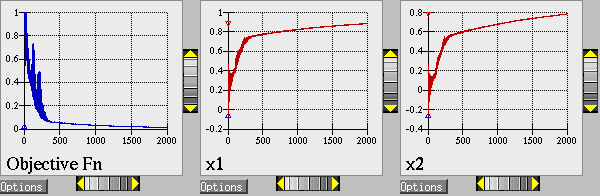
\includegraphics[width=\textwidth]{images/dak_graphics_ps_opt}}\\
  \multicolumn{2}{c}{(a)}\\
  \qquad\\
  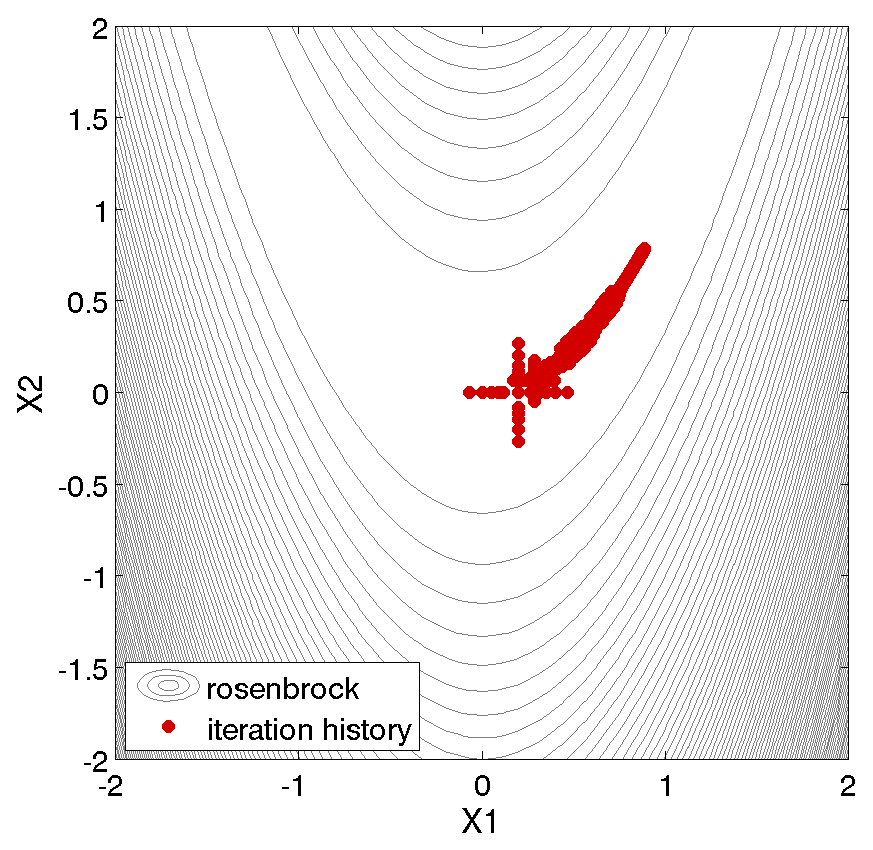
\includegraphics[height=2.5in]{images/rosen_ps_opt_pts} &
  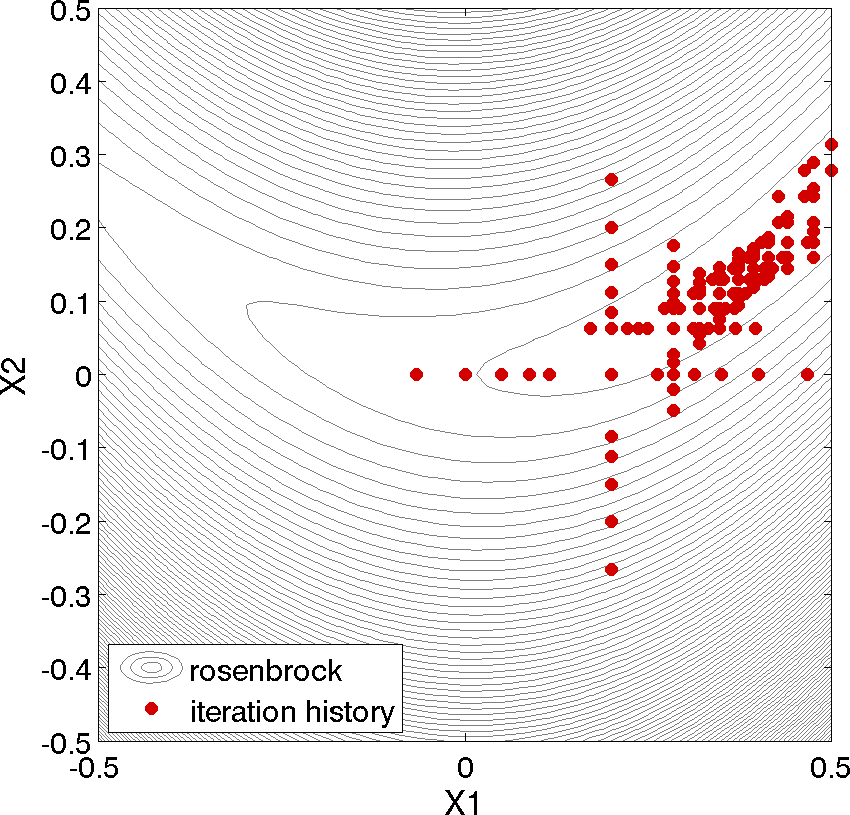
\includegraphics[height=2.5in]{images/rosen_ps_opt_pts2} \\
  (b) & (c)
  \end{tabular}
  \caption{Rosenbrock pattern search optimization example: (a) screen
    capture of the legacy Dakota X windows-based graphics, (b)
    sequence of design points (dots) evaluated and (c) close-up view
    illustrating the shape of the coordinate pattern used. }
  \label{opt:methods:gradientfree:local:example:ps_graphics}
\end{figure}

While pattern search algorithms are useful in many optimization
problems, this example shows some of the drawbacks to this algorithm.
While a pattern search method may make good initial progress towards
an optimum, it is often slow to converge. On a smooth, differentiable
function such as Rosenbrock's function, a nongradient-based method
will not be as efficient as a gradient-based method. However, there
are many engineering design applications where gradient information is
inaccurate or unavailable, which renders gradient-based optimizers
ineffective. Thus, pattern search algorithms are often good choices in
complex engineering applications when the quality of gradient data is
suspect.

\subsection{Derivative-Free Global Methods}
\label{opt:methods:gradientfree:global}

The discussion of derivative-free global methods is identical to that
in~\ref{opt:methods:gradientfree:local}, so we forego repeating it
here.  There are two types of global optimization methods in Dakota.

\subsubsection{Method Descriptions}
\label{opt:methods:gradientfree:global:descriptions}

{\bf Evolutionary Algorithms (EA)} are based on Darwin's theory of
survival of the fittest. The EA algorithm starts with a randomly
selected population of design points in the parameter space, where the
values of the design parameters form a ``genetic string,'' analogous
to DNA in a biological system, that uniquely represents each design
point in the population. The EA then follows a sequence of
generations, where the best design points in the population (i.e.,
those having low objective function values) are considered to be the
most ``fit'' and are allowed to survive and reproduce. The EA
simulates the evolutionary process by employing the mathematical
analogs of processes such as natural selection, breeding, and
mutation. Ultimately, the EA identifies a design point (or a family of
design points) that minimizes the objective function of the
optimization problem. An extensive discussion of EAs is beyond the
scope of this text, but may be found in a variety of sources (cf.,
~\cite{Haf92} pp. 149-158;~\cite{Gol89}). EAs available in Dakota
include \texttt{coliny\_ea}, \texttt{soga}, and \texttt{moga}.  The
latter is specifically designed for multi-objective problems,
discussed further in~\ref{opt:additional}.  All variants can optimize
over discrete variables, including discrete string variables, in
addition to continuous variables.  We note that an experimental branch
and bound capability is being matured to provide a gradient-based
approach to solving mixed variable global optimization problems.  One
key distinction is that it does not handle categorical variables
(e.g., string variables).  The branch and bound method is discussed
further in Section~\ref{adv_meth:minlp}.

{\bf DIvision of RECTangles (DIRECT)}~\cite{Gab01} balances local
search in promising regions of the design space with global search in
unexplored regions.  It adaptively subdivides the space of feasible
design points to guarantee that iterates are generated in the
neighborhood of a global minimum in finitely many iterations.  Dakota
includes two implementations (\texttt{ncsu\_direct} and
\texttt{coliny\_direct}.  In practice, DIRECT has proven an effective
heuristic for many applications.  For some problems, the
\texttt{ncsu\_direct} implementation has outperformed the
\texttt{coliny\_direct} implementation.  \texttt{ncsu\_direct} can
accommodate only bound constraints, while \texttt{coliny\_direct}
handles nonlinear constraints using a penalty formulation of the
problem.

{\bf Efficient Global Optimization (EGO)} is a global optimization
technique that employs response surface surrogates~\cite{Jon98,Hua06}.
In each EGO iteration, a Gaussian process (GP) approximation for the
objective function is constructed based on sample points of the true
simulation.  The GP allows one to specify the prediction at a new
input location as well as the uncertainty associated with that
prediction.  The key idea in EGO is to maximize an Expected
Improvement Function (EIF), defined as the expectation that any point
in the search space will provide a better solution than the current
best solution, based on the expected values and variances predicted by
the GP model.  It is important to understand how the use of this EIF
leads to optimal solutions.  The EIF indicates how much the objective
function value at a new potential location is expected to be less than
the predicted value at the current best solution.  Because the GP
model provides a Gaussian distribution at each predicted point,
expectations can be calculated.  Points with good expected values and
even a small variance will have a significant expectation of producing
a better solution (exploitation), but so will points that have
relatively poor expected values and greater variance (exploration).
The EIF incorporates both the idea of choosing points which minimize
the objective and choosing points about which there is large
prediction uncertainty (e.g., there are few or no samples in that area
of the space, and thus the probability may be high that a sample value
is potentially lower than other values).  Because the uncertainty is
higher in regions of the design space with few observations, this
provides a balance between exploiting areas of the design space that
predict good solutions, and exploring areas where more information is
needed.

There are two major differences between our implementation and that of
~\cite{Jon98}: we do not use a branch and bound method to find points
which maximize the EIF.  Rather, we use the DIRECT algorithm.  Second,
we allow for multiobjective optimization and nonlinear least squares
including general nonlinear constraints.  Constraints are handled
through an augmented Lagrangian merit function approach (see
Surrogate-Based Minimization chapter in Dakota Theory
Manual~\cite{TheoMan}).

\subsubsection{Examples}
\label{opt:methods:gradientfree:global:example}

{\bf Evolutionary algorithm:} In contrast to pattern search
algorithms, which are local optimization methods, evolutionary
algorithms (EA) are global optimization methods. As was described
above for the pattern search algorithm, the Rosenbrock function is not
an ideal test problem for showcasing the capabilities of evolutionary
algorithms. Rather, EAs are best suited to optimization problems that
have multiple local optima, and where gradients are either too
expensive to compute or are not readily available.

\begin{figure}[ht!]
  \centering
  \begin{bigbox}
    \begin{small}
      \verbatimtabinput[8]{rosen_opt_ea.in}
    \end{small}
  \end{bigbox}
  \caption{Rosenbrock evolutionary algorithm optimization example: the
  Dakota input file --
see \protect\path{dakota/share/dakota/examples/users/rosen_opt_ea.in} }
  \label{opt:methods:gradientfree:global:example:rosenbrock_ea}
\end{figure}

Figure~\ref{opt:methods:gradientfree:global:example:rosenbrock_ea}
shows a Dakota input file that uses an EA to minimize the Rosenbrock
function. For this example the EA has a population size of 50. At the
start of the first generation, a random number generator is used to
select 50 design points that will comprise the initial
population. \emph{[A specific seed value is used in this example to
  generate repeatable results, although, in general, one should use
  the default setting which allows the EA to choose a random seed.]} A
two-point crossover technique is used to exchange genetic string
values between the members of the population during the EA breeding
process. The result of the breeding process is a population comprised
of the 10 best ``parent'' design points (elitist strategy) plus 40 new
``child'' design points. The EA optimization process will be
terminated after either 100 iterations (generations of the EA) or
2,000 function evaluations. The EA software available in Dakota
provides the user with much flexibility in choosing the settings used
in the optimization process. See~\cite{RefMan} and~\cite{Har06} for
details on these settings.

The EA optimization results printed at the end of this file show that
the best design point found was $(x_1,x_2) = (0.98,0.95)$. The file
\path{ea_tabular.dat.sav} provides a listing of the design
parameter values and objective function values for all 2,000 design
points evaluated during the running of the EA. Figure~
\ref{opt:methods:gradientfree:global:example:rosenbrock_ea_graphics}(a)
shows the population of 50 randomly selected design points that
comprise the first generation of the EA, and
Figure~\ref{opt:methods:gradientfree:global:example:rosenbrock_ea_graphics}(b)
shows the final population of 50 design points, where most of the 50
points are clustered near $(x_1,x_2) = (0.98,0.95)$.

\begin{figure}[hbt!]
  \centering
  \begin{tabular}{cc}
  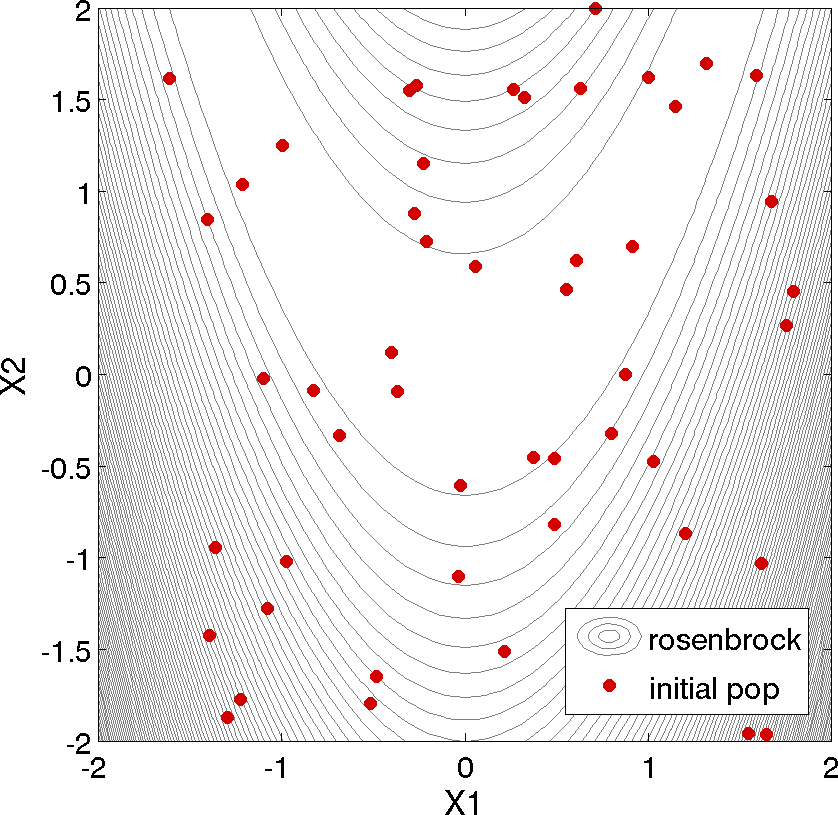
\includegraphics[height=2.5in]{images/rosen_ea_init} &
  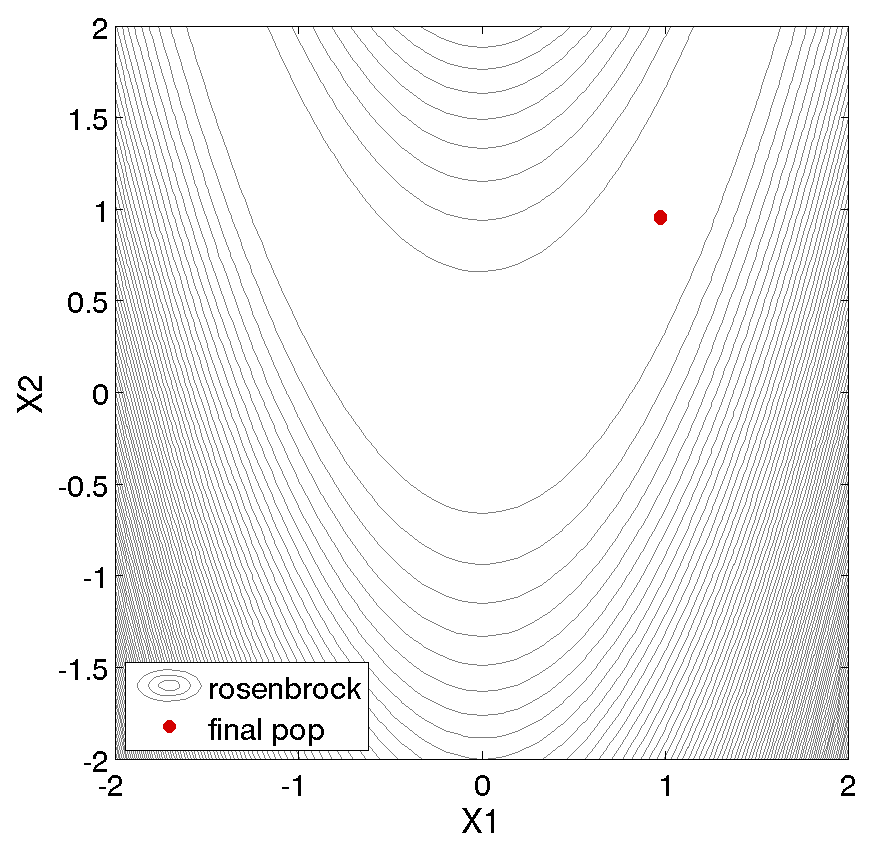
\includegraphics[height=2.5in]{images/rosen_ea_final} \\
  (a) & (b)
  \end{tabular}
  \caption{Rosenbrock evolutionary algorithm optimization example: 50
    design points in the (a) initial and (b) final populations
    selected by the evolutionary algorithm. }
  \label{opt:methods:gradientfree:global:example:rosenbrock_ea_graphics}
\end{figure}

As described above, an EA is not well-suited to an optimization
problem involving a smooth, differentiable objective such as the
Rosenbrock function. Rather, EAs are better suited to optimization
problems where conventional gradient-based optimization fails, such as
situations where there are multiple local optima and/or gradients are
not available. In such cases, the computational expense of an EA is
warranted since other optimization methods are not applicable or
impractical. In many optimization problems, EAs often quickly identify
promising regions of the design space where the global minimum may be
located. However, an EA can be slow to converge to the optimum. For
this reason, it can be an effective approach to combine the global
search capabilities of a EA with the efficient local search of a
gradient-based algorithm in a \emph{hybrid optimization} strategy. In
this approach, the optimization starts by using a few iterations of a
EA to provide the initial search for a good region of the parameter
space (low objective function and/or feasible constraints), and then
it switches to a gradient-based algorithm (using the best design point
found by the EA as its starting point) to perform an efficient local
search for an optimum design point. More information on this hybrid
approach is provided in Section~\ref{adv_meth:hybrid}.

{\bf Efficient Global Optimization:} The method is specified as
\texttt{efficient\_global}.  Currently we do not expose any
specification controls for the underlying Gaussian process model used
or for the optimization of the expected improvement function, which is
currently performed by the NCSU DIRECT algorithm. The only item the
user can specify is a seed which is used in the Latin Hypercube
Sampling to generate the initial set of points which is used to
construct the initial Gaussian process.  An example specification for
the EGO algorithm is shown in Figure~\ref{opt:methods:gradientfree:global:example:egm_rosen}.
\begin{figure}
  \begin{bigbox}
    \begin{small}
      \verbatimtabinput[8]{rosen_opt_ego.in}
    \end{small}
  \end{bigbox}
  \caption{Dakota input file for the efficient global optimization example --
see \protect\path{dakota/share/dakota/examples/users/rosen_opt_ego.in} }
  \label{opt:methods:gradientfree:global:example:egm_rosen}
\end{figure}


\section{Additional Optimization Capabilities}
\label{opt:additional}

Dakota provides several capabilities which extend the services
provided by the optimization software packages described in
Sections~\ref{opt:methods:gradient}
through~\ref{opt:methods:gradientfree:global}. Those described in this
section include:
\begin{itemize}
\item {\bf Multiobjective optimization}: There are three capabilities
  for multiobjective optimization in Dakota. The first is MOGA,
  described above in
  Section~\ref{opt:methods:gradientfree:global:descriptions}. The
  second is the Pareto-set strategy, described in
  Section~\ref{adv_meth:pareto}. The third is a weighting factor approach for
  multiobjective reduction, in which a composite objective function is
  constructed from a set of individual objective functions using a
  user-specified set of weighting factors. These latter two approaches
  work with any of the above single objective algorithms.
\item {\bf Scaling,} where any optimizer (or least squares solver
  described in Section~\ref{nls:solution}), can accept user-specified
  (and in some cases automatic or logarithmic) scaling of continuous
  design variables, objective functions (or least squares terms), and
  constraints. Some optimization algorithms are sensitive to the
  relative scaling of problem inputs and outputs, and this feature can
  help.
% \item {\bf Solvers in shared libraries}: On computer systems that
%   permit use of shared libraries (most modern systems), Dakota can
%   avail itself of optimization solvers contained in shared libraries.
%   This is a first step toward allowing optional parts of Dakota, such
%   as proprietary solvers, to be accessed from shared
%   libraries.
\end{itemize}
The Advanced Methods Chapter~\ref{adv_meth} offers details on the 
following component-based meta-algorithm approaches:
\begin{itemize}
\item \textbf{Sequential Hybrid Minimization}: This meta-algorithm
  allows the user to specify a sequence of minimization methods, with
  the results from one method providing the starting point for the
  next method in the sequence. An example which is useful in many
  engineering design problems involves the use of a nongradient-based
  global optimization method (e.g., genetic algorithm) to identify a
  promising region of the parameter space, which feeds its results
  into a gradient-based method (quasi-Newton, SQP, etc.) to perform an
  efficient local search for the optimum point.

\item \textbf{Multistart Local Minimization}: This meta-algorithm uses
  many local minimization runs (often gradient-based), each of which
  is started from a different initial point in the parameter
  space. This is an attractive approach in situations where multiple
  local optima are known to exist or may potentially exist in the
  parameter space. This approach combines the efficiency of local
  minimization methods with the parameter space coverage of a global
  stratification technique.

\item \textbf{Pareto-Set Minimization}: The Pareto-set minimization
  strategy allows the user to specify different sets of weights for
  either the individual objective functions in a multiobjective
  optimization problem or the individual residual terms in a least
  squares problem. Dakota executes each of these weighting sets as a
  separate minimization problem, serially or in parallel, and then
  outputs the set of optimal designs which define the Pareto
  set. Pareto set information can be useful in making trade-off
  decisions in engineering design problems.
\end{itemize}

\subsection{Multiobjective Optimization}
\label{opt:additional:multiobjective}

Multiobjective optimization refers to the simultaneous optimization of
two or more objective functions. Often these are competing objectives,
such as cost and performance. The optimal design in a multi-objective
problem is usually not a single point. Rather, it is a set of points
called the Pareto front. Each point on the Pareto front satisfies the
Pareto optimality criterion, which is stated as follows: a feasible
vector $X^{*}$ is Pareto optimal if there exists no other feasible
vector $X$ which would improve some objective without causing a
simultaneous worsening in at least one other objective. Thus, if a
feasible point $X'$ exists that CAN be improved on one or more
objectives simultaneously, it is not Pareto optimal: it is said to be
``dominated'' and the points along the Pareto front are said to be
``non-dominated.''

There are three capabilities for multiobjective optimization in
Dakota. First, there is the MOGA capability described previously in
Section~\ref{opt:methods:gradientfree:global:descriptions}. This is a
specialized algorithm capability. The second capability involves the
use of response data transformations to recast a multiobjective
problem as a single-objective problem. Currently, Dakota supports the
simple weighted sum approach for this transformation, in which a
composite objective function is constructed from a set of individual
objective functions using a user-specified set of weighting
factors. This approach is optimization algorithm independent, in that
it works with any of the optimization methods listed previously in
this chapter.  The third capability is the Pareto-set meta-algorithm
described in Section~\ref{adv_meth:pareto}. This capability also
utilizes the multiobjective response data transformations to allow
optimization algorithm independence; however, it builds upon the basic
approach by computing sets of optima in order to generate a Pareto
trade-off surface.

In the multiobjective transformation approach in which multiple
objectives are combined into one, an appropriate single-objective
optimization technique is used to solve the problem. The advantage of
this approach is that one can use any number of optimization methods
that are especially suited for the particular problem class. One
disadvantage of the weighted sum transformation approach is that a
linear weighted sum objective will only find one solution on the
Pareto front.  Since each optimization of a single weighted objective
will find only one point near or on the Pareto front, many
optimizations need to be performed to get a good parametric
understanding of the influence of the weights.  Thus, this approach
can become computationally expensive.

A multiobjective optimization problem is indicated by the
specification of multiple ($R$) objective functions in the responses
keyword block (i.e., the \texttt{objective\_functions} specification
is greater than \texttt{1}). The weighting factors on these objective
functions can be optionally specified using the \texttt{weights}
keyword (the default is equal weightings $\frac{1}{R}$). The composite
objective function for this optimization problem, $F$, is formed using
these weights as follows: $F=\sum_{k=1}^{R}w_{k}f_{k}$, where the
$f_{k}$ terms are the individual objective function values, the
$w_{k}$ terms are the weights, and $R$ is the number of objective
functions. The weighting factors stipulate the relative importance of
the design concerns represented by the individual objective functions;
the higher the weighting factor, the more dominant a particular
objective function will be in the optimization process. Constraints
are not affected by the weighting factor mapping; therefore, both
constrained and unconstrained multiobjective optimization problems can
be formulated and solved with Dakota, assuming selection of an
appropriate constrained or unconstrained single-objective optimization
algorithm. When both multiobjective weighting and scaling are active,
response scaling is applied prior to weighting.

\subsubsection{Multiobjective Example 1}
\label{opt:additional:multiobjective:example1}

Figure~\ref{opt:additional:multiobjective:example1:figure01} shows a
Dakota input file for a multiobjective optimization problem based on
the ``textbook'' test problem.  In the standard textbook formulation,
there is one objective function and two constraints. In the
multiobjective textbook formulation, all three of these functions are
treated as objective functions (\texttt{objective\_functions = 3}),
with weights given by the \texttt{weights} keyword. Note that it is
not required that the weights sum to a value of one. The
multiobjective optimization capability also allows any number of
constraints, although none are included in this example.

\begin{figure}
\centering
\begin{bigbox}
\begin{small}
\verbatimtabinput[8]{textbook_opt_multiobj1.in}
\end{small}
\end{bigbox}
\caption{Example Dakota input file for multiobjective optimization --
see \protect\path{dakota/share/dakota/examples/users/textbook_opt_multiobj1.in} }
\label{opt:additional:multiobjective:example1:figure01}
\end{figure}

Figure~\ref{opt:additional:multiobjective:example1:figure02} shows an
excerpt of the results for this multiobjective optimization problem,
with output in verbose mode. The data for function evaluation 9 show
that the simulator is returning the values and gradients of the three
objective functions and that this data is being combined by Dakota
into the value and gradient of the composite objective function, as
identified by the header ``\texttt{Multiobjective
  transformation:}''. This combination of value and gradient data from
the individual objective functions employs the user-specified
weightings of \texttt{.7}, \texttt{.2}, and \texttt{.1}. Convergence
to the optimum of the multiobjective problem is indicated in this case
by the gradient of the composite objective function going to zero (no
constraints are active).

\begin{figure}
\centering
\begin{bigbox}
\begin{small}
\begin{verbatim}
   ------------------------------
   Begin Function Evaluation    9
   ------------------------------
   Parameters for function evaluation 9:
                         5.9388064483e-01 x1
                         7.4158741198e-01 x2

   (text_book /tmp/fileFNNH3v /tmp/fileRktLe9)
   Removing /tmp/fileFNNH3v and /tmp/fileRktLe9

   Active response data for function evaluation 9:
   Active set vector = { 3 3 3 } Deriv vars vector = { 1 2 }
                         3.1662048106e-02 obj_fn_1
                        -1.8099485683e-02 obj_fn_2
                         2.5301156719e-01 obj_fn_3
    [ -2.6792982175e-01 -6.9024137415e-02 ] obj_fn_1 gradient
    [  1.1877612897e+00 -5.0000000000e-01 ] obj_fn_2 gradient
    [ -5.0000000000e-01  1.4831748240e+00 ] obj_fn_3 gradient



   -----------------------------------
   Post-processing Function Evaluation
   -----------------------------------
   Multiobjective transformation:
                         4.3844693257e-02 obj_fn
    [  1.3827084219e-06  5.8620632776e-07  ] obj_fn gradient

       7    1 1.0E+00    9  4.38446933E-02 1.5E-06    2 T TT     

    Exit NPSOL - Optimal solution found.

    Final nonlinear objective value =   0.4384469E-01
\end{verbatim}
\end{small}
\end{bigbox}
\caption{Dakota results for the multiobjective optimization example.}
\label{opt:additional:multiobjective:example1:figure02}
\end{figure}

By performing multiple optimizations for different sets of weights, a
family of optimal solutions can be generated which define the
trade-offs that result when managing competing design concerns. This
set of solutions is referred to as the Pareto set.
Section~\ref{adv_meth:pareto} describes an algorithm for
directly generating the Pareto set in order to investigate the
trade-offs in multiobjective optimization problems.

\subsubsection{Multiobjective Example 2}
\label{opt:additional:multiobjective:example2}

This example illustrates the use of multi-objective optimization based
on a genetic algorithm method. This method is called \texttt{moga}. It
is based on the idea that as the population evolves in a GA, solutions
that are non-dominated are chosen to remain in the population.  The
MOGA algorithm has separate fitness assessment and selection operators
called the \texttt{domination\_count} fitness assessor and
\texttt{below\_limit} selector respectively.  This approach of
selection works especially well on multi-objective problems because it
has been specifically designed to avoid problems with aggregating and
scaling objective function values and transforming them into a single
objective. Instead, the fitness assessor works by ranking population
members such that their resulting fitness is a function of the number
of other designs that dominate them. The \texttt{below\_limit}
selector then chooses designs by considering the fitness of each. If
the fitness of a design is above a certain limit, which in this case
corresponds to a design being dominated by more than a specified
number of other designs, then it is discarded. Otherwise it is kept
and selected to go to the next generation. The one catch is that this
selector will require that a minimum number of selections take
place. The \texttt{shrinkage\_percentage} determines the minimum
number of selections that will take place if enough designs are
available. It is interpreted as a percentage of the population size
that must go on to the subsequent generation. To enforce this, the
\texttt{below\_limit} selector makes all the selections it would make
anyway and if that is not enough, it relaxes its limit and makes
selections from the remaining designs. It continues to do this until
it has made enough selections.  The moga method has many other
important features. Complete descriptions can be found in the Dakota
Reference Manual~\cite{RefMan}.
 
We demonstrate the MOGA algorithm on three examples that are taken
from a multiobjective evolutionary algorithm (MOEA) test suite
described by Van Veldhuizen et. al. in~\cite{Coe02}. These three
examples illustrate the different forms that the Pareto set may
take. For each problem, we describe the Dakota input and show a graph
of the Pareto front. These problems are all solved with the
\texttt{moga} method.  The first example is presented below, the other
two examples are presented in the additional examples chapter
~\ref{additional:multiobjective:problem2} and
~\ref{additional:multiobjective:problem3}.

In Van Veldhuizen's notation, the set of all Pareto optimal design
configurations (design variable values only) is denoted $\mathtt{P^*}$
or $\mathtt{P_{true}}$ and is defined as:
\begin{eqnarray*}
  P^*:=\{x\in\Omega\,|\,\neg\exists\,\,
  x^\prime\in\Omega\quad\bar{f}(x^\prime)\preceq\bar{f}(x)\}
\end{eqnarray*}
 
The Pareto front, which is the set of objective function values
associated with the Pareto optimal design configurations, is denoted
$\mathtt{PF^*}$ or $\mathtt{PF_{true}}$ and is defined as:
\begin{eqnarray*}
  PF^*:=\{\bar{u}=\bar{f}=(f_1(x),\ldots,f_k(x))\,|\, x\in P^*\}
\end{eqnarray*}
 
The values calculated for the Pareto set and the Pareto front using
the moga method are close to but not always exactly the true values,
depending on the number of generations the moga is run, the various
settings governing the GA, and the complexity of the Pareto set.
 
The first test problem is a case where $P_{true}$ is connected and
$PF_{true}$ is concave. The problem is to simultaneously optimize
$f_1$ and $f_2$ given three input variables, $x_1$, $x_2$, and $x_3$,
where the inputs are bounded by $-4 \leq x_{i} \leq 4$:
 
Figure~\ref{opt:additional:multiobjective:example2:moga1inp} shows an
input file that demonstrates some of the multi-objective capabilities
available with the moga method.
\begin{figure}[htp!]
  \centering
  \begin{bigbox}
    \begin{small}
      \verbatimtabinput[8]{mogatest1.in}
    \end{small}
  \end{bigbox}
  \caption{Multiple objective genetic algorithm (MOGA) example: the
    Dakota input file --
see \protect\path{dakota/share/dakota/examples/users/mogatest1.in} }
  \label{opt:additional:multiobjective:example2:moga1inp}
\end{figure}
 
In this example, the three best solutions (as specified by
\texttt{final\_solutions} =3) are written to the output. Additionally,
final results from moga are output to a file called
\path{finaldata1.dat} in the directory in which you are
running. This \path{finaldata1.dat} file is simply a list of inputs
and outputs. Plotting the output columns against each other allows one
to see the Pareto front generated by \texttt{moga}.
Figure~\ref{opt:additional:multiobjective:example2:moga_pareto} shows
an example of the Pareto front for this problem. Note that a Pareto
front easily shows the trade-offs between Pareto optimal solutions. For
instance, look at the point with f1 and f2 values equal to (0.9,
0.23). One cannot improve (minimize) the value of objective function
f1 without increasing the value of f2: another point on the Pareto
front, (0.63, 0.63) represents a better value of objective f1 but a
worse value of objective f2.
\begin{figure}[ht!]
  \centering
  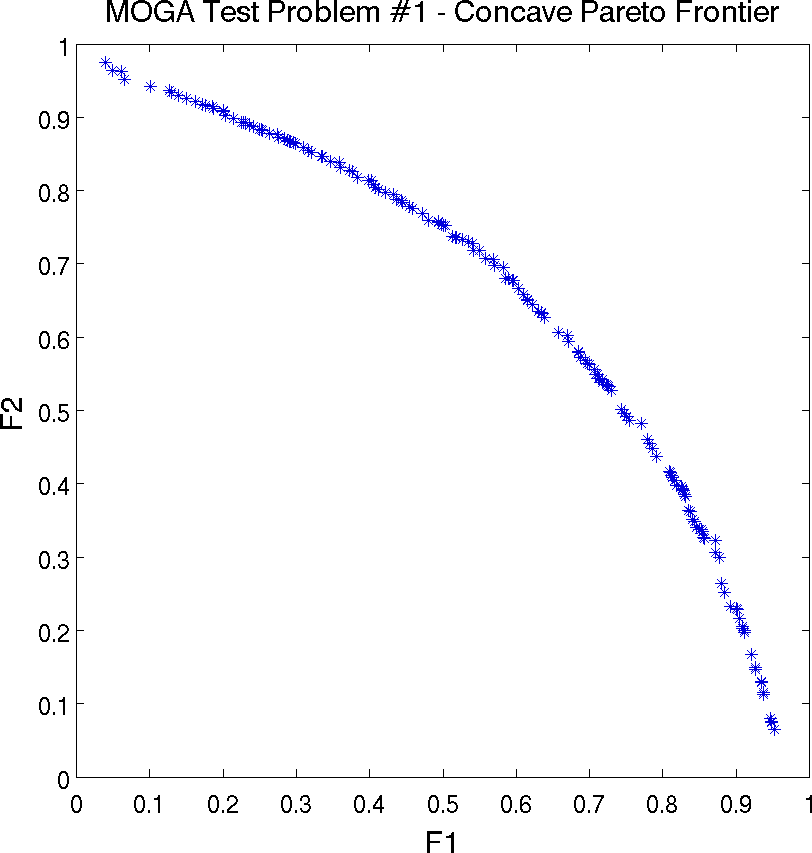
\includegraphics[scale=0.75]{images/dakota_mogatest1_pareto_front}
  \caption{Multiple objective genetic algorithm (MOGA) example: Pareto
  front showing trade-offs between functions f1 and f2.}
  \label{opt:additional:multiobjective:example2:moga_pareto}
\end{figure}


\subsection{Optimization with User-specified or Automatic Scaling}
\label{opt:additional:scaling}

Some optimization problems involving design variables, objective
functions, or constraints on vastly different scales may be solved
more efficiently if these quantities are adjusted to a common scale
(typically on the order of unity). With any optimizer (or least
squares solver described in Section~\ref{nls:solution}),
user-specified characteristic value scaling may be applied to any of
continuous design variables, functions/residuals, nonlinear inequality
and equality constraints, and linear inequality and equality
constraints. Automatic scaling is available for variables or responses
with one- or two-sided bounds or equalities and may be combined with
user-specified scaling values. Logarithmic ($\log_{10}$) scaling is
available and may also be combined with characteristic values. Log
scaling is not available for linear constraints. Moreover, when
continuous design variables are log scaled, linear constraints are not
permitted in the problem formulation. Discrete variable scaling is not
supported.

Scaling is enabled on a per-method basis for optimizers and
calibration (least squares and Bayesian) methods by including the
\dakotakw{scaling} keyword in the relevant \dakotakw{method}
specification in the Dakota input file. When scaling is enabled,
variables, functions, gradients, Hessians, etc., are transformed such
that the optimizer iterates in the scaled variable/response space,
whereas evaluations of the computational model as specified in the
interface are performed on the original problem scale. Therefore using
scaling does not require rewriting the interface to the simulation
code. When the \dakotakw{scaling} keyword is absent, all other scale
type and value specifications described below are ignored in the
corresponding method, variables, and responses sections. When the
method's \dakotakw{output} level is set above normal, scaling
initialization and diagnostic information will be printed.

Scaling for a particular variable or response type is enabled through
the \dakotakw{*scale_types} and/or \dakotakw{*scales} specifications
(see the Reference Manual method section and references contained
therein for a complete keyword list). Valid options for the
string-valued \dakotakw{*scale_types} specifications include {\tt
  'value'}, {\tt 'auto'}, or {\tt 'log'}, for characteristic value,
automatic, or logarithmic scaling, respectively (although not all
types are valid for scaling all entities). If a single string is
specified with any of these keywords it will apply to each component
of the relevant vector, e.g., with \dakotakw{continuous_design = 3},
\dakotakw{scale_types = 'value'} will enable characteristic value
scaling for each of the 3 continuous design variables.

One may specify no, one, or a vector of characteristic scale values
through the \dakotakw{*scales} specifications.  These characteristic
values are required for {\tt 'value'}, and optional for {\tt 'auto'}
and {\tt 'log'}. If scales are specified, but not scale types, value
scaling is assumed. As with types, if a single value is specified with
any of these keywords it will apply to each component of the relevant
vector, e.g., if \dakotakw{scales = 3.4} is specified for continuous
design variables, Dakota will apply a characteristic scaling value of
3.4 to each continuous design variable.

When scaling is enabled, the following procedures determine the
transformations used to scale each component of a variables or
response vector. A warning is issued if scaling would result in
division by a value smaller in magnitude than {\tt 1.0e10*DBL\_MIN}.
User-provided values violating this lower bound are accepted
unaltered, whereas for automatically calculated scaling, the lower
bound is enforced.

\begin{itemize}

\item No \dakotakw{*scales} and no \dakotakw{*scale_types} specified
  for this component (variable or response type: no scaling performed
  on this component.

\item Characteristic value ({\tt 'value'}): the corresponding quantity
  is scaled (divided) by the required characteristic value provided in
  the corresponding \dakotakw{*scales} specification, and bounds are
  adjusted as necessary. If the value is negative, the sense of
  inequalities are changed accordingly.

\item Automatic ({\tt 'auto'}): First, any characteristic values from
  the optional corresponding \dakotakw{*scales} specification are
  applied. Then, automatic scaling will be attempted according to the
  following scheme:

  \begin{itemize}
  
  \item two-sided bounds scaled into the interval [0,1];
	
  \item one-sided bounds or targets are scaled by a characteristic
    value to move the bound or target to 1, and the sense of
    inequalities are changed if necessary;

  \item no bounds or targets: no automatic scaling possible for this component
    
  \end{itemize}

  Automatic scaling is not available for objective functions nor least
  squares terms since they lack bound constraints. Further, when
  automatically scaled, linear constraints are scaled by
  characteristic values only, not affinely scaled into [0,1].

\item Logarithmic ({\tt 'log'}): First, any characteristic values from
  the optional \dakotakw{*scales} specification are applied. Then,
  $\log_{10}$ scaling is applied. Logarithmic scaling is not available
  for linear constraints. Further, when continuous design variables
  are log scaled, linear constraints are not allowed.

\end{itemize}

Scaling for linear constraints specified through
\dakotakw{linear_inequality_scales} or
\dakotakw{linear_equality_scales} is applied {\em after} any
(user-specified or automatic) continuous variable scaling. For
example, for scaling mapping unscaled continuous design variables $x$
to scaled variables $\tilde{x}$:
\[ \tilde{x}^j = \frac{x^j - x^j_O}{x^j_M}, \]
where $x^j_M$ is the final component multiplier and $x^j_O$ the
offset, we have the following matrix system for linear inequality
constraints
\begin{eqnarray*}
& a_L \leq A_i x \leq a_U \\
& a_L \leq A_i \left( \mathrm{diag}(x_M) \tilde{x} + x_O \right) \leq a_U \\
& a_L - A_i x_O \leq A_i \mathrm{diag}(x_M) \tilde{x} \leq a_U - A_i x_O \\
& \tilde{a}_L \leq \tilde{A}_i \tilde{x} \leq \tilde{a}_U,
\end{eqnarray*}
and user-specified or automatically computed scaling multipliers are
applied to this final transformed system, which accounts for any
continuous design variable scaling. When automatic scaling is in use
for linear constraints they are linearly scaled by characteristic
values only, not affinely scaled into the interval $[0,1]$.

\subsubsection{Scaling Example}
\label{opt:additional:scaling:example}

Figure~\ref{opt:additional:scaling:example:figure01} demonstrates the
use of several scaling keywords for the textbook optimization problem.
The continuous design variable {\tt x1} is scaled by a characteristic
value of 4.0, whereas {\tt x2} is scaled automatically into $[0,1]$
based on its bounds. The objective function will be scaled by a factor
of 50.0, then logarithmically, the first nonlinear constraint by a
factor of 15.0, and the second nonlinear constraint is not scaled.

\begin{figure}
\centering
\begin{bigbox}
\begin{small}
\verbatimtabinput[8]{rosen_opt_scaled.in}
\end{small}
\end{bigbox}
\caption{Sample usage of scaling keywords in Dakota input specification --
see \protect\path{dakota/share/dakota/examples/users/rosen_opt_scaled.in} }
\label{opt:additional:scaling:example:figure01}
\end{figure}

%\subsection{dl\_solver --- Solvers via Shared Libraries}
%\label{opt:additional:dlsolver}
%
%On computer systems that permit use of shared libraries (most modern
%systems), Dakota can avail itself of optimization solvers contained in
%shared libraries.  This is a first step toward allowing optional parts
%of Dakota, such as proprietary solvers, to be accessed from shared
%libraries. For example, the Dakota source distributions illustrate
%making a sample shared-library interface to SNOPT~\cite{GilMS05},
%whose use would be specified by
%\begin{small}
%\begin{verbatim}
%    method,
%          dl_solver = 'dl_snopt.dll'
%\end{verbatim}
%\end{small}
%The quoted string contains the name of the shared library, optionally
%followed by keyword assignments known to the library, such as
%\begin{small}
%\begin{verbatim}
%    method,
%          dl_solver = 'dl_snopt.dll outlev = 1'
%\end{verbatim}
%\end{small}
%which would turn on some diagnostic printing in the SNOPT example.

\section{Optimization Usage Guidelines}
\label{opt:usage}

In selecting an optimization method, important considerations include
the type of variables in the problem (continuous, discrete, mixed),
whether a global search is needed or a local search is sufficient, and
the required constraint support (unconstrained, bound constrained, or
generally constrained). Less obvious, but equally important,
considerations include the efficiency of convergence to an optimum
(i.e., convergence rate) and the robustness of the method in the
presence of challenging design space features (e.g., nonsmoothness).

Table~\ref{opt:usage:guideopt} provides a convenient reference for
choosing an optimization method or strategy to match the
characteristics of the user's problem, where blank fields inherit the
value from above. With respect to constraint support, it should be
understood that the methods with more advanced constraint support are
also applicable to the lower constraint support levels; they are
listed only at their highest level of constraint support for brevity.

\begin{table}[hbp]
\centering
\caption{Guidelines for optimization method selection.} 
\label{opt:usage:guideopt}\vspace{2mm}
\begin{tabular}{|c|c|c|}
\hline
\textbf{Method} & \textbf{Desired Problem} & \textbf{Applicable Methods} \\
\textbf{Classification} & \textbf{Characteristics} & \\
\hline
Gradient-Based Local & smooth; continuous variables; no constraints
& optpp\_cg, rol \\
\hline
         & smooth; continuous variables; & dot\_bfgs, dot\_frcg \\
         & bound constraints & conmin\_frcg, rol \\
\hline
         & smooth; continuous variables; & npsol\_sqp, nlpql\_sqp, dot\_mmfd, \\
         & bound constraints, & dot\_slp, dot\_sqp,
         conmin\_mfd, \\
         & linear and nonlinear constraints & optpp\_newton,
         optpp\_q\_newton, \\
         &          &optpp\_fd\_newton, rol \\
         &          & weighted sums (multiobjective), \\
         &          & pareto\_set strategy (multiobjective) \\
\hline
Gradient-Based Global & smooth; continuous variables; & hybrid\_strategy, \\
         &  bound constraints, & multi\_start strategy \\
         &  linear and nonlinear constraints & \\
\hline
Derivative-Free Local & nonsmooth; continuous variables; bound constraints
& optpp\_pds \\
\hline
         & nonsmooth; continuous variables; & coliny\_cobyla,  \\
         & bound constraints, & coliny\_pattern\_search, \\
         & nonlinear constraints & coliny\_solis\_wets, \\
\hline
         & nonsmooth; continuous variables; & asynch\_pattern\_search, \\
         & bound constraints, & surrogate\_based\_local \\
         & linear and nonlinear constraints & \\
\hline
         & nonsmooth; continuous variables; &  \\
         & discrete variables; bound constraints, & mesh\_adaptive\_search \\
         & nonlinear constraints &  \\
\hline
Derivative-Free Global & nonsmooth; continuous variables; bound constraints
& ncsu\_direct \\
\hline
         & nonsmooth; continuous variables; & coliny\_direct,  \\
         & bound constraints, & efficient\_global \\
         & nonlinear constraints & \\
\hline
         & nonsmooth; continuous variables; & surrogate\_based\_global \\
         & bound constraints, &  \\
         & linear and nonlinear constraints & \\
\hline
         & nonsmooth; continuous variables, & coliny\_ea \\
         & discrete variables; bound constraints, &  \\
         & nonlinear constraints & \\
\hline
         & nonsmooth; continuous variables, & soga, \\
         & discrete variables; bound constraints, & moga (multiobjective) \\
         & linear and nonlinear constraints & \\
\hline
\end{tabular}
\end{table}

{\bf Gradient-based Methods} \\
Gradient-based optimization methods are highly efficient, with the
best convergence rates of all of the optimization methods. If analytic
gradient and Hessian information can be provided by an application
code, a full Newton method will provide quadratic convergence rates
near the solution. More commonly, only gradient information is
available and a quasi-Newton method is chosen in which the Hessian
information is approximated from an accumulation of gradient data. In
this case, superlinear convergence rates can be obtained. First-order
methods, such as the Method of Feasible Directions, may achieve only
a linear rate of convergence, which may entail more iterations, 
but potentially at a lower cost per iteration associated with 
Hessian calculations. These characteristics make gradient-based optimization
the methods of choice when the problem is smooth, unimodal, and
well-behaved. However, when the problem exhibits nonsmooth,
discontinuous, or multimodal behavior, these methods can also be the
least robust since inaccurate gradients will lead to bad search
directions, failed line searches, and early termination, and the
presence of multiple minima will be missed.

Thus, for gradient-based optimization, a critical factor is the
gradient accuracy. Analytic gradients are ideal, but are often
unavailable. For many engineering applications, a finite difference
method will be used by the optimization algorithm to estimate gradient
values. Dakota allows the user to select the step size for these
calculations, as well as choose between forward-difference and
central-difference algorithms. The finite difference step size should
be selected as small as possible, to allow for local accuracy and
convergence, but not so small that the steps are ``in the noise.''
This requires an assessment of the local smoothness of the response
functions using, for example, a parameter study method. Central
differencing, in general, will produce more reliable gradients than
forward differencing, but at roughly twice the expense.

ROL has traditionally been developed and applied to problems with 
analytic gradients (and Hessians). Nonetheless, ROL can be used with 
Dakota-provided finite-differencing approximations to the gradient of both 
objective and constraints. However, a user relying on such approximations 
is advised to resort to alternative optimizers such as DOT until performance 
of ROL improves in future releases.

We offer the following recommendations in deciding upon a 
suitable gradient-based method for a given problem
\begin{itemize}
\item For {\bf unconstrained and bound-constrained problems}, conjugate 
gradient-based methods exhibit the best scalability for large-scale 
problems (1,000+ variables). These include the Polak-Ribiere conjugate 
gradient method (\texttt{optpp\_cg}), ROL's trust-region method with 
truncated conjugate gradient subproblem solver (\texttt{rol}), and the 
Fletcher-Reeves conjugate gradient method (\texttt{conmin\_frcg} and 
\texttt{dot\_frcg}). These methods also provide good performance for 
small- to intermediate-sized problems. Note that due to performance 
issues, users relying on finite-differencing approximations to the gradient 
of the objective function are advised to resort to alternative optimizers 
such as DOT until performance of ROL improves in future releases.
\item For {\bf constrained problems}, with large number of constraints 
with respect to number of variables, Method of Feasible Directions 
methods (\texttt{conmin\_mfd} and \texttt{dot\_mmfd}) and Sequential 
Quadratic Programming methods (\texttt{nlpql\_sqp} and 
\texttt{npsol\_sqp}) exhibit good performance (relatively fast 
convergence rates). \emph{Note that we have observed weak convergence 
rates while using {\rm \texttt{npsol\_sqp}} for certain problems with 
equality constraints}. Quasi-Newton method \texttt{optpp\_q\_newton} 
show moderate performance for constrained problems across all scales.

\end{itemize}

{\bf Non-gradient-based Methods} \\
Nongradient-based methods exhibit much slower convergence rates for
finding an optimum, and as a result, tend to be much more
computationally demanding than gradient-based methods. Nongradient
local optimization methods, such as pattern search algorithms, often
require from several hundred to a thousand or more function
evaluations, depending on the number of variables, and nongradient
global optimization methods such as genetic algorithms may require
from thousands to tens-of-thousands of function evaluations. Clearly,
for nongradient optimization studies, the computational cost of the
function evaluation must be relatively small in order to obtain an
optimal solution in a reasonable amount of time. In addition,
nonlinear constraint support in nongradient methods is an open area of
research and, while supported by many nongradient methods in Dakota,
is not as refined as constraint support in gradient-based
methods. However, nongradient methods can be more robust and more
inherently parallel than gradient-based approaches. They can be
applied in situations were gradient calculations are too expensive or
unreliable. In addition, some nongradient-based methods can be used
for global optimization which gradient-based techniques, by
themselves, cannot. For these reasons, nongradient-based methods
deserve consideration when the problem may be nonsmooth, multimodal,
or poorly behaved.

{\bf Surrogate-based Methods} \\ Approaches that seek to improve the
effectiveness or efficiency of optimizers and least squares methods
through the use of surrogate models include the surrogate-based local,
surrogate-based global, and efficient global
methods. Section~\ref{adv_meth:sbm} provides further information on
these approaches. The surrogate-based local approach (see
Section~\ref{adv_meth:sbm:sblm}) brings the efficiency of
gradient-based optimization/least squares methods to nonsmooth or
poorly behaved problems by smoothing noisy or discontinuous response
results with a data fit surrogate model (e.g., a quadratic polynomial)
and then minimizing on the smooth surrogate using efficient
gradient-based techniques. The surrogate-based global approach (see
Section~\ref{adv_meth:sbm:sbgm}) similarly employs optimizers/least
squares methods with surrogate models, but rather than localizing
through the use of trust regions, seeks global solutions using global
methods.  And the efficient global approach (see
Section~\ref{opt:methods:gradientfree:global}) uses the specific combination of
Gaussian process surrogate models in combination with the DIRECT
global optimizer. Similar to these surrogate-based approaches, the
hybrid and multistart optimization component-based algorithms seek to bring the
efficiency of gradient-based optimization methods to global
optimization problems. In the former case, a global optimization
method can be used for a few cycles to locate promising regions and
then local gradient-based optimization is used to efficiently converge
on one or more optima. In the latter case, a stratification technique
is used to disperse a series of local gradient-based optimization runs
through parameter space. Without surrogate data smoothing, however,
these strategies are best for smooth multimodal
problems. Section~\ref{adv_meth:hybrid} and
Section~\ref{adv_meth:multistart} provide more information on these
approaches.

\section{Optimization Third Party Libraries}
\label{opt:libraries}

As mentioned in~\ref{opt}, Dakota serves as a delivery vehicle for a
number third-party optimization libraries. The packages are listed
here along with the license status and web page where available.

\begin{itemize}

\item CONMIN (\texttt{conmin\_} methods) License: Public Domain
  (NASA).

\item DOT (\texttt{dot\_} methods) License: commercial; website:
  Vanderplaats Research and Development,
  \url{http://www.vrand.com}. {\em Not included in the open source
    version of Dakota.  Sandia National Laboratories and Los Alamos
    National Laboratory have limited seats for DOT. Other users may
    obtain their own copy of DOT and compile it with the Dakota source
    code.}

\item HOPSPACK (\texttt{asynch\_pattern\_search}) License: LGPL; web
  page: \url{https://software.sandia.gov/trac/hopspack}.

\item JEGA (\texttt{soga}, \texttt{moga}) License: LGPL

\item NCSUOpt (\texttt{ncsu\_direct}) License: MIT

\item NLPQL (\texttt{nlpql\_} methods) License: commercial; website:
  Prof. Klaus Schittkowski,
  \url{http://www.uni-bayreuth.de/departments/math/~kschittkowski/nlpqlp20.htm}). \emph{Not included in the open source version of Dakota.  Users may
    obtain their own copy of NLPQLP and compile it with the Dakota
    source code.}

\item NPSOL (\texttt{npsol\_} methods) License: commercial; website:
  Stanford Business Software
  \url{http://www.sbsi-sol-optimize.com}. {\em Not included in the
    open source version of Dakota.  Sandia National Laboratories,
    Lawrence Livermore National Laboratory, and Los Alamos National
    Laboratory all have site licenses for NPSOL. Other users may
    obtain their own copy of NPSOL and compile it with the Dakota
    source code.}

\item NOMAD (\texttt{mesh\_adaptive\_search}) License: LGPL; website:
  \url{http://www.gerad.ca/NOMAD/Project/Home.html}.

\item OPT++ (\texttt{optpp\_} methods) License: LGPL; website:
  \url{http://csmr.ca.sandia.gov/opt++}.

\item ROL (\texttt{rol}) License: BSD; website:
  \url{https://trilinos.org/packages/rol}.

\item SCOLIB (\texttt{coliny\_} methods) License: BSD; website:
  \url{https://software.sandia.gov/trac/acro/wiki/Packages}.

\end{itemize}


%%  LocalWords:  equalities optimizers Hessians affinely unscaled
%%  LocalWords:  logarithmically
